% !TEX root = ../../../main.tex
% !TEX encoding = UTF-8 Unicode
% !TEX encoding = UTF-8

\section{Verfahren für die Kosten- und Zeitschätzung - BB, SH}
% \textit{Autoren: Benedikt Buchner, Sebastian Hanna}
\label{section_verfahren_schaetzung} % referenz zu KL
Nachdem in Kapitel \ref{section_kostenarten} die für diese Arbeit relevanten Kostenarten 
beleuchtet wurden, werden im Folgenden Möglichkeiten aufgezeigt, um die Kosten 
und die zur Realisierung benötigte Zeit zu schätzen. Im weiteren Verlauf werden 
Planungs- und Überwachungsin-strumente des Projektmanagements erläutert, die für 
das durchzuführende Projekt am geeignetsten scheinen. Dabei liegt der Fokus vor 
allem auf einer möglichst agilen Umsetzung des Projekts. Abschließend werden 
die untersuchten Verfahren beispielhaft auf drei konkrete Komponenten des Projekts 
angewendet.

% !TEX root = ../../../main.tex
% !TEX encoding = UTF-8 Unicode
% !TEX encoding = UTF-8

\subsection{Projektmanagement an einer Hochschule}
\label{subsection_projektmanagement_hochschule}
Wie bereits in Kapitel \ref{chapter_grundlagen_INM} beschrieben, weist eine Hochschule als Organisation eine Reihe von Besonderheiten auf. Für das Projektmanagement bedeutet besonders die Tatsache, dass die einzelnen Fachbereiche ein hohes Maß an Autonomie und Entscheidungskompetenzen besitzen, eine entsprechend angepasste Herangehensweise.\footcite{hansen_business_2009}

Die zentrale Herausforderung des Projektmanagements ist es, die Interessen der unterschiedlichen Verwaltungsbereiche, der späteren Nutzer und der Hochschulleitung zu wahren und zu vereinen. Durch die Autonomie der Fachbereiche und deren unterschiedlichen Interessen ist es möglich, dass sich innerhalb der Hochschule konkurrierende Arbeitsgruppen bilden. Es ist daher eine weitere, nicht zu unterschätzende, Aufgabe des Projektmanagements, die Kommunikation zwischen allen beteiligten Arbeitsgruppen, möglichen externen Akteuren und dem akademischen Bereich aufrecht zu erhalten und zu fördern.\footcite{altvater_organisation_2007}

Des Weiteren führen umfangreiche Änderungen in Organisationen oftmals zu einer besonderen Eigendynamik, die, im Zusammenspiel mit den aufgeführten Besonderheiten einer Hochschule, zu nicht kalkulierbaren oder unvorhersehbaren Geschehnissen führen können. Der Umstand, dass zu Projektbeginn in der Regel noch nicht alle, für eine exakte Planung benötigten, Informationen zur Verfügung stehen, erschwert zusätzlich die zufriedenstellende Organisation des Projektverlaufs. Um dem entgegen zu wirken ist es empfehlenswert, dass Projekt in iterativ-reflexiven Schleifen mit ausreichender Flexibilität durchzuführen.\footcite{hansen_business_2009}

Durch die gewonnene Flexibilität sind Anpassungen während der Ausführung des Projektes möglich und auf besondere Befindlichkeiten kann eingegangen werden. Durch eine iterative Durchführung wird außerdem dem Vorhaben Rechnung getragen, dass nach jeder Umsetzung einer Komponente über den weiteren Verlauf des Projekts reflektiert werden kann.


% !TEX root = ../../../main.tex
% !TEX encoding = UTF-8 Unicode
% !TEX encoding = UTF-8

\subsection{Kostenschätzung (Total Cost of Ownership) - SH}
% \textit{Autor: Sebastian Hanna}

\label{subsection_kostenschatzung_TCO}
Neben der Organisation und Durchführung des Projekts bildet die Schätzung der Kosten im Vorfeld 
eine weitere wichtige Säule des Projektmanagements. Eine möglichst ganzheitliche und realistische 
Erfassung aller potentiell entstehenden Kosten ist dabei notwendig, um die Entscheidung für oder 
gegen ein Projekt anhand fundierter Informationen treffen zu können.

Das Total-Cost-Of-Ownership-Konzept wurde im Rahmen einer Studie der Gartner Group 
zur vollständigen Erfassung der direkten und indirekten Kosten eines PC-Arbeitsplatzes 
entwickelt. Das Ergebnis der Studie hat dabei gezeigt, dass nur ca. 20\% der Gesamtkosten 
tatsächlich auf die direkten Anschaffungskosten von Hard- und Software entfallen. 

Der Großteil der entstehenden Kosten wird folglich durch den Einführungsprozess neuer 
Systeme und den langfristigen Betrieb selbiger verursacht. Der Einsatz der TCO-Methode 
kann demnach dabei helfen, ein Bewertungsobjekt mit allen zugehörigen, 
kostenverursachenden Aspekten zu erfassen und zu bewerten.\footnote{\cite{hansen_business_2009}}

Die Tatsache, dass es sich bei dem untersuchten Studienobjekt lediglich um einen “wenig komplexen” PC-Arbeitsplatz handelt, lässt vermuten, dass bei Einführung komplexer Systeme (z.B. Dokumentenmanagement) der Anteil der Anschaffungskosten über den gesamten Lebenszyklus des Systems weiter schrumpft, während Inbetriebnahme, Wartung und Schulung wesentlich mehr Kosten verursachen. Dieser Zusammenhang verdeutlicht die Wichtigkeit der ganzheitlichen Kostenbetrachtung und rechtfertigt den Einsatz des TCO-Konzepts, das es zum Ziel hat, den Vollständigkeitsgrundsatz der Kostenrechnung\footnote{\cite{grob_einfuhrung_2004}} zu erfüllen.

Grundsätzlich wird im Falle der TCO-Analyse zwischen direkten und indirekten, bzw. budgetierten und nicht-budgetierten, Kosten unterschieden. In die Kategorie der direkten Kosten fallen alle Investitionen, die zur Beschaffung und Bereitstellung der IT-Komponente notwendig sind. Die Bezeichnung als budgetierte Kosten liegt darin begründet, dass selbige einem konkreten Bereich (z.B. Hochschulrechenzentrum) zugeschrieben werden können. Im Gegensatz dazu handelt es sich bei indirekten Kosten um Ausgaben, die außerhalb des Bereichs auftreten, der die direkten Kosten zu tragen hat, wodurch sie keinem konkreten Budget zugeschrieben werden können. Eine generische Übersicht der direkten und indirekten Kategorien zeigt Abbildung \ref{fig_generische_kostenarten} \footnote{\cite{hansen_business_2009}}.

\begin{figure}[h!]
	\centering
	\includegraphics[width=\textwidth]
	{kapitel/gruppe4_2/bilder/generische_kostenkategorien}
	\caption{generische Kostenkategorien und -arten, nach Hansen}
	\label{fig_generische_kostenarten}
\end{figure}

Während die im Diagramm dargestellten direkten Kosten auch direkt in der IT-Abteilung anfallen und nachvollziehbar, beziehungsweise durch angemessenen Aufwand berechenbar, sind, entstehen die indirekten Kosten in der Regel durch Endanwender und deren “unsachgemäße Nutzung” der bereitgestellten Infrastruktur. Dies ist theoretisch bereits dann der Fall, wenn ein Mitarbeiter einen anderen Mitarbeiter bei der Lösung von IT-Problemen unterstützt, obwohl dies nicht seine eigentliche Aufgabe ist. Durch diese Arbeiten außerhalb seines Zuständigkeitsbereichs werden die eigentlichen Kernaktivitäten des Mitarbeiters vernachlässigt, wodurch seine Produktivität sinkt. Dieser Produktivitätsverlust wird durch sogenannte Opportunitätskosten abgebildet und als indirekte Kostenstelle erfasst.

Die Erhebung der Informationen, die notwendig sind, um indirekte Kosten beziffern zu können, kann sich jedoch als äußerst schwierig und zeitaufwendig herausstellen. Aufgrund fehlender formalisierter Techniken zur Erfassung eben dieser Positionen, empfiehlt die Gartner Group den Einsatz von Befragungen und Fokusgruppen, was neben dem bereits erwähnten, hohen zeitlichen Aufwand, außerdem zu Problemen hinsichtlich der Validität der Daten führen kann.\footnote{\cite{hansen_business_2009}}

Ferner besteht die Gefahr, dass durch die Berücksichtigung von Opportunitätskosten der in Kapitel \ref{subsection_projektmanagement_hochschule} beschriebene, notwendige Austausch und Kontakt zwischen verschiedenen Arbeitsgruppen und Fachbereichen stark eingeschränkt wird. Deshalb sollte in diesem speziellen, nicht-industriellen, Fall einer Hochschule auf die initiale Berücksichtigung der indirekten Kosten verzichtet werden. Im späteren Projektverlauf, nachdem das Zusammenspiel aller Akteure etabliert und gefestigt ist, muss jedoch versucht werden, diese Daten zu evaluieren und in die Kalkulation mit einzubeziehen.

Eine beispielhafte Kalkulation auf Grundlage der TCO-Methode der Gartner Group wird in Kapitel \ref{subsubsection_dokusystem_alfresco} durchgeführt. Als unterstützende Software zur Berechnung dient die kostenlose Anwendung TCO-Tool.\footnote{\url{http://sourceforge.net/projects/tcotool/}}

% !TEX root = ../../../main.tex
% !TEX encoding = UTF-8 Unicode
% !TEX encoding = UTF-8

\subsection{Zeitplanung - BB}
% \textit{Autor: Benedikt Buchner}

Neben der Einschätzung der zu erwarteten Kosten soll der zeitliche Ablauf der einzelnen Projektkomponenten beleuchtet werden. Die aufsummierte Dauer der einzelnen Komponenten ergibt dann den gesamten zeitlichen Aufwand Projekts. Zur zeitlichen Planung der erforderlichen Schritte, sowie der Ablaufplanung einzelner Arbeitspakete werden Gantt-Diagramme eingesetzt. Die Anwendung eines solchen Gantt-Diagramms stellt das erste Kapitel dieses Abschnitts dar. Die Einhaltung der zuvor definierten Meilensteine und Arbeitsschritte wird dabei anhand der Meilensteintrendanalyse durchgeführt. Wie die Meilensteintrendanalyse zur Überwachung der Projektmodule eingesetzt werden soll wird im zweiten Teil dieses Kapitels erklärt.

\subsubsection{Gantt-Diagramm}
Zur Erstellung eines Gantt-Diagramms ist es wichtig, zunächst eine Aktivitätenliste zu erstellen, die durch das Zerlegen von Arbeitspaketen generiert wird. Eine Möglichkeit diese Arbeitspakete zu ermitteln besteht im Erstellen eines Projektstrukturplans. Eine Aktivität erhält dabei, neben Metainformationen, wie einer eindeutigen Nummer und der Person der diese Aktivität zugwiesen wird, für die zeitliche Planung entscheidende Parameter wie der genauen Dauer dieser Aktivität und einer möglichen Wartezeit die vor oder nach dem Abarbeiten selbiger eintritt.\footnote{\cite{kraus_projekt_2010}}  Da das Schätzen der benötigten Zeit zur Bearbeitung einer Aktivität im Kontext dieses Projekts stark von Erfahrungen abhängt, sollen hierzu Experten bezüglich dieser Erfahrungswerte befragt werden.

Die Darstellung eines Gantt-Diagramms unterliegt keinen gestalterischen Vorgaben oder Richtlinien und sind für alle Ebenen der Planung einsetzbar. Jede Aktivität muss lediglich durch einen Balken dargestellt werden, dessen Länge proportional zu der Dauer der Aktivität ist.\footnote{\cite{jakoby_intensivtraining_2015}}

Ein großer Vorteil dieser Diagrammart ist die Übersichtlichkeit, da es durch den Aufbau des Diagramms möglich ist, auf einen Blick zu erkennen wann welche Aktivität begonnen werden und wann diese beendet sein muss. Ein Nachteil ist die Tatsache, dass mögliche Abhängigkeiten nicht aufgezeigt werden können.\footnote{\cite{kraus_projekt_2010}}

Die zuvor aus den Aufgabenpaketen ermittelten Aktivitäten werden also in das Gantt-Diagramm übertragen und mit entsprechenden Balken versehen. Dies wird in Abbildung \ref{fig_beispiel_gantt_diagramm} verdeutlicht:

\begin{figure}[h!]
	\centering
	\includegraphics[width=\textwidth]
	{kapitel/gruppe4_2/bilder/beispiel_gantt_diagramm}
	\caption{Beispiel eines Gantt-Diagramms}
	\label{fig_beispiel_gantt_diagramm}
\end{figure}

Die Aktivitäten werden, wie das Beispiel zeigt, vertikal erfasst. Die horizontale Achse bildet den zeitlichen Ablauf ab. Sie ist frei definierbare Zeiteinheiten, hier Tage, unterteilt. Den einzelnen Aktivitäten wurde in Abhängigkeit ihrer Dauer ein jeweils entsprechend langer Balken zugeordnet.

Es gilt zu beachten, dass für jede Komponente die innerhalb des Projekts umgesetzt werden soll, ein solches Diagramm erstellt wird. Damit wird der hohen Modularität des Projekts Rechnung getragen und eine entsprechend agile Priorisierung der umzusetzenden Komponenten ist möglich. Die Reihenfolge der Umsetzung ist somit frei wählbar, ohne dabei die Möglichkeit einer zeitlichen Planung bei der Umsetzung innerhalb Komponente zu verlieren.

\subsubsection{Meilensteintrendanalyse}
Die Meilensteintrendanalyse (MTA) ist ein wichtiges und dabei einfach anzuwendendes Werkzeug zur Überwachung essentieller Projekttermine. In diesem Zusammenhang werden Projekttermine auch Meilensteine genannt. Die MTA liefert dabei zwei grundlegende Informationen: Einerseits liefert sie einen Überblick über die Entwicklung zukünftiger Termine, andererseits lässt sich anhand dieser Entwicklung die Stabilität der Terminprognosen erkennen.\footnote{\cite{gadatsch_masterkurs_2014}}

Abbildung \ref{fig_MTA_diagramme} zeigt exemplarisch den Aufbau eines MTA-Diagramms:
\begin{figure}[h!]
	\centering
	\includegraphics[width=\textwidth]{kapitel/gruppe4_2/bilder/mta_diagramme}
	\caption{Mögliche Ausprägungen der MTA Diagramme}
	\label{fig_MTA_diagramme}
\end{figure}

In der Abbildung \ref{fig_MTA_diagramme} ist zu erkennen, dass ein MTA-Diagramm zwei Dimensionen besitzt. Auf der horizontalen Achse werden die Berichtstermine in vorher vereinbarten und regelmäßigen Abständen aufgetragen. Die vertikale Achse ist mit den geplanten Projekterminen (Meilensteinen) beschriftet. Die Schnittstellen der Achsen geben das aktuelle, möglicherweise korrigierte Fälligkeitsdatum des Meilensteins zum Zeitpunkt des Berichts an. In jedem Bericht müssen die Meilensteintermine neu bewertet werden. Dabei ist es irrelevant ob der Termin sich nach hinten verschiebt, der Termin dem der letzten Beurteilung entspricht oder das geplante Datum unterschritten werden kann. Die Ergebnisse dieser Beurteilungen werden in dem Diagramm eingetragen, woraus sich im Laufe des Projekts Kurven ergeben. Diese Kurven entsprechen in der Regel einem der drei typischen Verläufe. Fallende Kurven zeigen, dass die Termine initial zu pessimistisch geschätzt wurden und häufig nach unten korrigiert werden mussten. Steigende Kurven bedeuten hingegen, dass Termine zu optimistisch geschätzt wurden. Die weitestgehend gerade verlaufenden Kurven stellen entsprechend den Idealverlauf dar.\footnote{\cite{gadatsch_masterkurs_2014}}

% !TEX root = ../../../main.tex
% !TEX encoding = UTF-8 Unicode
% !TEX encoding = UTF-8

\subsection{Anwendung - BB, SH}
% \textit{Autoren: Benedikt Buchner, Sebastian Hanna}
\label{kosten_zeit_anwendung} % bitte als Referenz drin lassen für KL
Nachdem die Werkzeuge zur zeitlichen und kostentechnischen Schätzung theoretisch beleuchtet wurden, werden diese im Folgenden beispielhaft auf ausgewählte Komponenten des Projekts angewendet. Für die Einführung des Dokumentenmanagementsystem Alfresco wird eine TCO-Analyse sowie ein Gantt-Diagramm angefertigt. Die potentiellen Kosten des Redesigns der Hochschulwebseite (inkl. der Anpassung  an moderne Ausgabegeräte) werden auf Grundlage von Gesprächen mit entsprechenden Experten analysiert. Die Berechnungen des Zeitbedarfs geht davon aus, dass die entsprechenden Komponenten des Projekts während des Semesters, also nicht zu besonders arbeitsintensiven Zeiten wie Prüfungsphasen am Ende oder Planungsphasen am Anfang eines Semesters, durchgeführt werden.

\subsubsection{Dokumentenmanagementsystem Alfresco}
\label{subsubsection_dokusystem_alfresco}
Um erfolgreich ein Dokumentenmanagementsystem (DMS) in einer Organisation einzuführen, müssen verschiedene Vorbedingungen erfüllt sein. Das betrifft neben dem erforderlichen Personal zur Einrichtung, technischer Wartung, den Help-Desk und inhaltlicher Pflege auch benötigte Hardware und Netzwerkinfrastruktur.

Um eine möglichst realitätsnahe Planung zu ermöglichen wurde hierzu Herr Stephan Voigt, aktuell CTO der Masterpayment AG, befragt. Herr Voigt hat bereits zahlreiche CMS Projekte, unter anderem die Einführung von Alfresco als DMS bei der Masterpayment AG, betreut, sodass seine Expertenmeinung verlässliche Zahlen ergibt. Diese Zahlen werden anschließend anhand der in Abschnitt \ref{subsection_kostenschatzung_TCO} beschriebenen TCO-Methode betrachtet. Die daraus resultierende Abbildung \ref{tab_ubersicht_kosten_TCO} stellt einen Überblick über die zu erwartenden Kosten dar. Folgende Bereiche wurden durch die Befragung beleuchtet:

\begin{itemize}
	\item Hardware für Anwenderprozesse und IT-Abteilung
	\item Software für Anwenderprozesse, Help-Desk und Incidentmanagement
	\item Prozessmanagement während des Betriebs durch Administartor(en)
	\item Wartungsarbeiten durch Administrator(en)
	\item Schulung der verantwortlichen Betreuer
	\item Erstellen von Anwenderhandbuch
\end{itemize}

Da dies eine beispielhafte Betrachtung ist, geht die Berechnung davon aus, dass alle aufgeführten Ressourcen angeschafft oder eingerichtet werden müssen. Sollte die Hochschule Teile dieser Ressourcen aus eigenem Bestand zur Verfügung stellen, müssen die Werte in der TCO Berechnung entsprechend angepasst werden.

\begin{figure}[h]
	\centering
	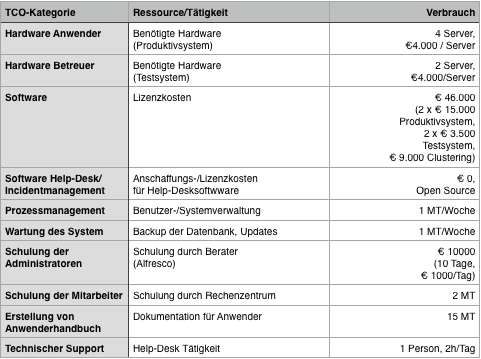
\includegraphics[width=\textwidth]
	{kapitel/gruppe4_2/bilder/uebersicht_kosten_tco_methode_neu}
	\caption{Übersicht der Kosten für die TCO-Methode}
	\label{tab_ubersicht_kosten_TCO}
\end{figure}

Die in Abbildung \ref{tab_ubersicht_kosten_TCO} erfassten Kosten werden in das, in Kapitel
\ref{subsection_kostenschatzung_TCO} erwähnte, TCO-Tool übertragen. 
Anhand der verfügbaren Analysefunktionen werden anschließend die Gesamtkosten nach den 
TCO-Kostenkategorien ausgegeben und aufgeschlüsselt. Das Ergebnis der Kalkulation anhand 
des TCO-Tools zeigt Tabelle \ref{tab_ergebnis_TCO_Methode}. Die Betrachtung erfolgt dabei, 
entsprechend der Abschreibungsdauer nach der DFG-Nutzungstabelle\footcite[Vgl.]{lmu_dfg_klassen_42}, über einen Zeitraum von 48 Monaten.

\begin{figure}[h]
	\centering
	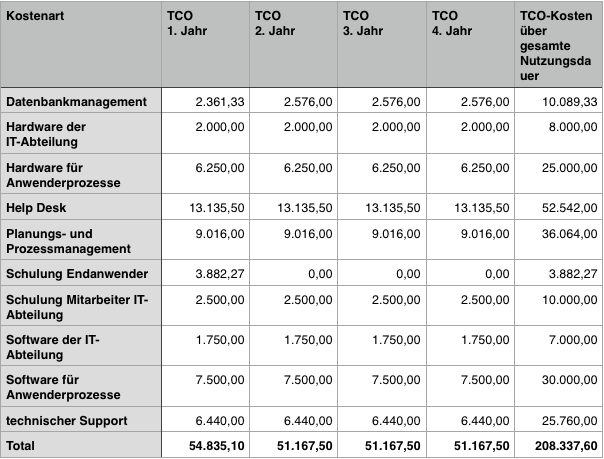
\includegraphics[width=\textwidth]
	{kapitel/gruppe4_2/bilder/tabelle_ergebnis_tco_methode}
	\caption{Ergebnis der TCO-Methode}
	\label{tab_ergebnis_TCO_Methode}
\end{figure}

Abbildung \ref{tab_ergebnis_TCO_Methode} zeigt den finanziellen, beziehungsweise zeitlichen, 
Aufwand der nach Einschätzung des befragten Experten nötig ist, um das 
Dokumentenmanagementsystem Alfresco an der Hochschule einzuführen und zu betreiben. 
Da in dem Interview mit dem Leiter des Rechenzentrums der Hochschule nicht geklärt werden 
konnte, in welchem Rahmen dem Gesamtprojekt vorhandene Hardware zur Verfügung gestellt 
werden kann, wird in dieser TCO-Analyse davon ausgegangen, dass Hardware angeschafft 
werden muss.

Aus Gründen der Hochverfügbarkeit wird Alfresco in einem Cluster betrieben. Dazu werden auf 
jeweils zwei Servern Alfresco und eine dazugehörige Datenbank eingerichtet. Die Server mit 
einer ausreichend performanteren Hardware liegen bei EUR 4.000 das Stück. Des Weiteren ist 
es ratsam, ein Testsystem zu installieren auf dem Updates oder zusätzliche 
Eigenimplementierungen getestet werden können. Da ein solches Testsystem nicht der gleichen 
Last wie das Produktivsystem ausgesetzt ist, ist es ausreichend zwei echte Server, auf denen jeweils 
zwei Server virtualisiert werden, zu verwenden. Auch diese Server werden mit je EUR 4.000 
veranschlagt.
\newpage

Alfresco bietet von ihrer DMS-Software eine kostenfreie Community-Version und eine lizenzpflichtige Kauf-Version an. Das größte Manko der Community-Version sind die nicht verfügbaren Aktualisierungen. Soll also eine bereits installierte Community-Version auf eine neue Softwareversion aktualisiert werden, muss das gesamte System neu aufgesetzt werden. Der Vorteil der regelmäßigen Aktualisierungen der kostenpflichtigen Version überwiegt also den Kostenvorteil der kostenfreie Softwarelösung.

Die Lizenzgebühren für die Software liegen jeweils bei ca. EUR 15.000 für die Produktivsysteme und EUR 3.500 für die Testsysteme. Dazu kommen Kosten in Höhe von ca. EUR 9.000 für Softwarekomponenten die den Betrieb im Cluster ermöglichen. Da es zahlreiche Open-Source Lösungen für den Betrieb eines Help-Desks, beziehungsweise eines Ticketsystems, gibt, fallen hierfür keine zusätzlichen Kosten an.

Nach der Installation läuft Alfresco zu einem großen Teil alleine und benötigt keine weitere Interaktion von außen. Es fallen ledigliche kleinere Wartungsarbeiten, wie das Einspielen von Aktualisierungen oder das Anfertigen einer Datenbanksicherung, an. Diese werden mit einem Aufwand von ca. 1 MT pro Woche veranschlagt. Dazu kommt die Verwaltung der Benutzer des Systems mit einem weiteren MT pro Woche. Da die Mitarbeiter des Rechenzentrums hauptsächlich für den Reibungslosen Betrieb der Plattform verantwortlich sein sollen, werden diese von Beratern der Alfresco Software AG geschult. Die Schulung ist mit 10 Tagen geplant und verursacht Kosten in Höhe von EUR 1.000 je Tag. Anwender des Systems können sich anschließend von den Mitarbeitern des Rechenzentrums schulen lassen. Für eine Anwenderschulung werden ca. 2 MT geplant. Zusätzlich wird ein Anwenderhandbuch erstellt. Die Erstellung dauert ca. 15 MT. Nach der Einführung des System wird sich ein Mitarbeiter des Help-Desks erfahrungsgemäß etwa 2 Stunden täglich mit Anliegen rund um Alfresco beschäftigen.

Die angenommenen Personalkosten entsprechen den Personalmittelsätzen für 2015 der DFG und beruhen auf “Bruttoarbeitgeberkosten”. Die Grundlage der Berechnung der Stundensätze bildet die Anzahl der Arbeitstage des Jahres 2016 unter Berücksichtigung von, entsprechend den Tarifen des öffentlichen Dienstes\footcite[Vgl.][]{tarife_ofd_42}, 30 Urlaubstagen und 39 Wochenstunden (insgesamt 224 Arbeitstage). Die angenommenen Stundensätze sind zur Wahrung der Transparenz nachfolgend in Tabelle \ref{tab_ubersicht_lohne} dargestellt.

\begin{table}[h!]
	%\begin{tabularx}{\textwidth}{|l|X|X|}
	\begin{tabularx}{\textwidth}{@{}l *2{>{\centering\arraybackslash}X}@{}}
		% Überschriften
		\hline \textbf{Personalkategorie} & \textbf{EUR / Jahr} & \textbf{EUR / Stunde}\\
		% Zeile 1
		Postdoktorand/in & 65.400 & 37,50 \\ 
		Doktorand/in & 60.600 & 34,70 \\
		Wissenschaftliche(r) Mitarbeiter/in & 51.500 & 29,20 \\
		Nichtwissenschaftliche(r) Mitarbeiter/in & 45.000 & 25,80 \\
		Studentische Hilfskraft &  & 13,65 \\
		\hline
	\end{tabularx}
	\caption{Übersicht der Jahres- und Stundenlöhne}
	\label{tab_ubersicht_lohne}
\end{table}
\clearpage

Der benötigte zeitliche Rahmen und der Ablauf der Einführung von Alfresco als Dokumentenmanagementsystems wird durch ein Gantt-Diagramm visualisiert. Die Daten für die Erstellung dieses Diagramms wurden ebenfalls im Rahmen der Expertenbefragung ermittelt.

\begin{figure}[h!]
	\centering
	\includegraphics[width=\textwidth]
	{kapitel/gruppe4_2/bilder/gantt_diagramm_alfresco}
	\caption{Gantt Diagramm Alfresco}
	\label{fig_gantt_diagramm_alfresco}
\end{figure}

Das Gantt-Diagramm in Abbildung \ref{fig_gantt_diagramm_alfresco} zeigt die Dauer der einzelnen Teilschritte der Einführung des Teilprojektes „Alfresco“. Die Gesamtdauer des Teilprojekts ist die Strecke zwischen dem Anfang des obersten und dem Ende des untersten Balkens. Die Datumsangaben sind hier zu ignorieren, es geht nur um die Gesamtzahl an Mitarbeiterinnen- und Mitarbeitertagen (im Folgenden als MT abgekürzt), die die Umsetzung des Teilprojekts benötigt. Im ersten Schritt müssen die Server sowohl für Test- als auch für die Produktivsysteme konfiguriert und in das vorhandene Netzwerk integriert werden. Danach wird die Software installiert und entsprechend den Vorgaben der Fachbereiche konfiguriert. Nach der Installation können die Administratoren des DMS geschult werden um in dem nächsten Schritt ein Handbuch erstellen zu können. Die Qualitätsicherung des Handbuches und des DMS folgt zum Abschluss des Projekts. Ingesamt dauert die Einführung 30 MT.

\subsubsection{Redesign / Relaunch Hochschule-Webseite}
\label{subsubsection_redesign_webseite}
Um den Aufwand - und damit auch den Kosten- und Zeitrahmen der Umsetzung einer neuen Hochschulwebsite zu ermitteln, wurden Gespräche mit mehreren Experten\footnote{Achim Gosse, Geschäftsführender Gesellschafter digitalnoise GmbH (\url{www.digitalnoise.de})}\footnote{Stefan Becker, Software- und Webentwickler (\url{www.beckeste.de})} geführt.

Die Ergebnisse dieser Gespräche finden sich zusammengefasst in Tabelle \ref{tab_aufwand_redesign}, die die verschiedenen Phasen des Entwicklungsprozesses, vom initialen Workshop bis hin zur Auslieferung und Qualitätsicherung, abbildet. Als Einheit wird dabei auf Mitarbeiterinnen- und Mitarbeitertage (im Folgenden als MT abgekürzt) statt auf monetäre Angaben gesetzt, da Stunden- und Tagessätze teils starken regionalen Unterschieden unterliegen. Es gilt zu beachten, dass die hier durchgeführte Betrachtung der Kosten lediglich die externen Kosten berücksichtigt. Ausfallzeiten von Mitarbeitern, die beispielsweise durch die Teilnahme an Workshops generiert werden, werden nicht berücksichtigt.

\begin{table}
	\centering
	\begin{tabularx}{10cm}{@{}l *1{>{\raggedleft\arraybackslash}X}@{}}
		\hline \textbf{Aufgabe} & \textbf{MT} \\
			Workshop & 5\\
			Konzept & 10\\
			Präsentation Konzept & 2\\
			User experience & 5\\
			Design & 15\\
			Präsentation Design & 2\\
			Endpräsentation & 3\\
			technische Umsetzung & 2\\
			Anpassung Content & 5\\
			Qualitätssicherung & 3\\
			Deployment & 1\\
			Puffer & 5\\
			\textbf{Gesamt} & \textbf{48 - 53}\\
			
		\hline
	\end{tabularx}
	\caption{Aufwandsschätzung zum Redesign der Hochschule-Webseite}
	\label{tab_aufwand_redesign}
\end{table}

Der Initiale Schritt des gesamten Prozesses sollte, sofern im Voraus kein ausgearbeitetes Konzept vorliegt, in der Durchführung von Workshops mit Entscheidungsträgern aus allen beteiligten Bereichen (Verwaltung, Fachbereiche, Rechenzentrum, etc.) liegen. Um das Ziel des Workshops, nämlich eine gemeinsame Grundlage zu schaffen, die von allen gleichermaßen getragen wird, zu erreichen, werden, bedingt durch das vorhandene Konfliktpotential, 5 MT zur Durchführung angesetzt.

Die Ergebnisse des Workshops werden anschließend durch Konzeptioner, die an dem Workshop als “Zuhörer” teilgenommen haben, verarbeitet, um daraus ein Website-Konzept zu entwickeln. Für die Ausarbeitung des Konzepts mit entsprechender Präsen-tation vor den Projektverantwortlichen der Hochschule werden 12 MT veranschlagt.

Nachdem das Konzept freigegeben wurde, können User-Experience-Experten und (User Interface-)Designer mit der Ausarbeitung der Gestaltungsvorlage beginnen. Dabei ist es üblich, dem Kunden mehrere, möglichst unterschiedliche, Designvorschläge zu unterbreiten. Inklusive Präsentation und Ausarbeitung des finalen Vorschlags kann dieser Posten mit 22 MT berechnet werden.

Auf Basis des verabschiedeten Designs kann die technische Realisierung der neuen Konzepte und Gestaltungsvorlagen beginnen. Da zum einen die benötigten Kompetenzen innerhalb der Hochschule vorhanden sind und zum anderen das interne Konfliktpotential in diesem Schritt wesentlich geringer ausfällt, bietet es sich an, diesen Schritt hochschulintern durchzuführen. 

Die kalkulierten 7 MT durch die Dienstleister setzen sich aus den Punkten “technische Umsetzung” (2 MT) und “Anpassung Content” (5 MT) zusammen. Die 2 MT der technischen Umsetzung sind dabei zur Unterstützung des Hochschulteams vorgesehen, während die 5 Tage vor allem genutzt werden, um auf “content-seitige” Sonderfälle reagieren zu können. Da bereits TYPO3 als Content Management System zum Einsatz kommt, sollte die Migration des bestehenden Inhalts in ein neues System entfallen. Durch die Möglichkeit des Multi-Channel-Publishings und Hilfsmittel zur Erstellung barrierearmer Websites ist ein Wechsel des Systems nicht erforderlich.

Vor der Auslieferung und dem “live gehen” des Internetauftritts steht noch die finale Qualitätssicherung. Dabei wird die gesamte Webpräsenz abschließend auf Konsistenz und Fehlerfreiheit geprüft. Bei einer Website diesen Umfangs werden für die Überprüfung und Korektur eventueller Fehler 3 MT berechnet.

Die eigentliche Auslieferung sollte nach der Qualitätssicherung innerhalb eines Arbeitstages durchgeführt sein. Zur Absicherung wird eine Arbeitswoche als Puffer veranschlagt, sodass die Umsetzung des Projekts im Kostenrahmen von 48 bis 53 MT liegt.

Da das Erstellen eines Konzepts für einen komplexen Internetauftritt im Allgemeinen mit einem nicht zu unterschätzenden Aufwand verbunden ist, wird ein solches Konzept durch die entsprechenden Agenturen in der Regel nur angefertigt, wenn dahinter die Aussicht auf den Erhalt des entsprechenden Auftrags steht. Da weder ein bestehendes Konzept, noch die konkrete Aussicht auf einen tatsächlichen Auftrag vorliegen, konnten durch die Dienstleister keine konkreten Angebote abgegeben werden.

\subsubsection{Facebook Seite}
Facebook unterscheidet verschiedene Arten von Applikationen die mit einem Profil verknüpft werden können. Dabei ist es unerheblich ob dieses Profil einer Privatperson, einem Unternehmen oder einer anderen Organisation zugeordnet wird.\footcite[Vgl.][]{dev_fb_42}

Die Hochschule Emden/Leer hat bereits ein reguläres Facebook Profil. Es gilt nun für die einzelnen Fachbereiche sogenannte “Page Tabs” einzurichten. “Page Tabs” werden auf einer Facebook Profil-Seite als Menü-Links eingeblendet. Der Inhalt der Tabs wird wird mit einer, nach speziellen Vorgaben gestalteten, Webseite in die Profil-Seite integriert. Facebook gibt mit einer API das Format vor. Auch die Nutzung anderer Elemente der Facebook Dienste bedarf einer Integration der Facebook API. Dabei ist zu beachten, dass die Webseite, deren Inhalt in dem Tab angezeigt wird, auf einem externen Server, in diesem Fall einem Server der Hochschule, liegt.\footcite[Vgl.][]{dev_fb_42}

Bei der Ermittlung des Zeitbedarfs für die Erstellung eines Tabs geht es folglich darum, den zeitlichen Aufwand für das Anfertigen einer regulären Webseite nach den Vorgaben der Facebook API zu schätzen. 

Die benötigten Funktionen einer solchen Webseite und der dazugehörige Entwicklungsaufwand werden wieder durch Befragung eines Experten ermittelt. Als Experte für dieses Teilprojekt stand Herr Dipl.-Inf. Franz Riehl von der jambit GmbH aus München zur Verfügung. Analog zur Kalkulation der Website in Kapitel \ref{subsubsection_redesign_webseite} wird auch in diesem Fall in Mitarbeiterinnen- und Mitarbeitertagen (im Folgenden als MT abgekürzt) gerechnet:

\begin{table}
	\centering
	\begin{tabularx}{10cm}{@{}l *1{>{\raggedleft\arraybackslash}X}@{}}
		\hline \textbf{Aufgabe} & \textbf{MT} \\
		Konzept & 1\\
		Design & 10\\
		Präsentation & 1\\
		Realisierung & 8\\
		Integration & 1\\
		Abnahme / QS & 1\\
		\textbf{Gesamt} & \textbf{22}\\
		
		\hline
	\end{tabularx}
	\caption{Aufwandsschätzung zur Entwicklung der "Facebook Page Tabs"}
	\label{tab_aufwand_facebook_page}
\end{table}

Der initiale Schritt besteht erneut in der Konzeption der einzubindenden Webanwendung. Da das Konzept der Page-Tabs für jeden Fachbereich identisch sein sollte, fällt der konzeptionelle Aufwand nur einmalig an. Das Konzept besteht in diesem Fall aus der Auswahl der zu transportierenden Informationen und einer entsprechenden Darstellungsform, wofür 1 MT kalku kalkuliert wird.

Im Gegensatz zum Konzept sollte die Gestaltung der Page-Tabs an den jeweiligen Fachbereich angepasst werden. Da es im Idealfall bereits ein Corporate-Design Manual gibt, in dem grundlegende Gestaltungsrichtlinien festgehalten sind, werden für diesen Schritt 2,5 Tage pro Fachbereich berechnet, sodass in Summe 10 MT berücksichtigt werden müssen.

Nach der Präsentation aller vier Designs, wofür 1 MT veranschlagt wird, folgt die Realisierung. Da die Gestaltung an die Fachbereiche angepasst wurde, können die Vorlagen voraussichtlich nicht alle nach dem gleichen Schema umgesetzt werden, weshalb für jeden Page-Tab 2 MT kalkuliert werden.

Die finalen Schritte bestehen in der Facebook-Integration mit abschließender Qualitäts-sicherung. Pro Fachbereich kann diesbezüglich ein halber MT vorge vorgesehen werden, sodass die letzten Punkte mit insgesamt 2 MT zu Buche schlagen. Die Gesamtsumme beträgt bei dem beschriebenen Vorgehen 22 MT.

Da es sich bei dem Facebook-Auftritt nicht um ein “kritisches System” im Sinne der Verfügbarkeit der Anwendung handelt, bietet es sich an, die Webanwendungen im Rahmen einer Projekt- oder Bachelorarbeit umsetzen zu lassen. Neben der Tatsache, dass so die Gestaltung und Umsetzung “direkt durch die Zielgruppe” des Auftritts geschieht, können dadurch Kosten eingespart werden. Alternativ sollte auf studentische Hilfskräfte zurückgegriffen werden.
\newpage

Eine exemplarische Kalkulation auf Grundlage der bereits in Kapitel \ref{subsubsection_dokusystem_alfresco} erfassten Stundensätze zeigt Tabelle \ref{tab_kosten_umsetzung_facebook}.

\begin{table}[h!]
	\centering
	\begin{tabularx}{\textwidth}{l|r|l|*1{>{\raggedleft\arraybackslash}X}@{}}
		\hline \textbf{Aufgabe} & \textbf{MT} & \textbf{Personalkostenkategorie} & \textbf{Betrag} \\
		Konzept & 1 & studentische Hilfskraft & 109,20\\
		Design & 10 & studentische Hilfskraft & 1092,00\\
		Präsentation & 0,5 & studentische Hilfskraft & 54,60\\
		 & 0,5 & Nichtwissenschaftlicher Mitarbeiter & 103,20\\
		Realisierung & 8 & studentische Hilfskraft & 873,60\\
		Integration & 1 & studentische Hilfskraft & 109,20\\
		Abnahme / QS & 1 & Nichtwissenschaftlicher MItarbeiter & 206,40\\
		\textbf{Gesamt} & \textbf{21,5} & & \textbf{1.565,40}\\
		
		\hline
	\end{tabularx}
	\caption{Exemplarische Kostenkalkulation der Umsetzung der "Facebook Page Tabs"}
	\label{tab_kosten_umsetzung_facebook}
\end{table}

Die Realisierung der Page-Tabs durch eine studentische Hilfskraft würde folglich ca. 350 Euro kosten. Da die Präsentation vermutlich vor einem nichtwissenschaftlichen Mitarbeiter gehalten wird, müssen auch dessen Personalkosten für den Zeitraum der Präsentation berücksichtigt werden. Ebenso erfolgt die Abnahme und Qualitätssicherung voraussichtlich durch einen nichtwissenschaftlichen Mitarbeiter.

